
\subsection{Model Setup}
\subsubsection{Model Domain}
The domain of the model is bounded by longitudes $\phi_E=-180^{\circ}$ and $\phi_W=-180^{\circ}$ and latitudes $\theta_N=80^{\circ}$ and $\theta_S=-80^{\circ}$ with periodic boundary conditions in the zonal direction.
 The depth profile has 15 layers with grid stretching (\cref{fig:gridstrech}). The grid stretching relation is such that surface layers are much shallower than deep water layers. There are $90 \times 40$ horizontal grid points to make a $4^{\circ} \times 4^{\circ}$ resolution model.
 
 \begin{figure}[H]
 	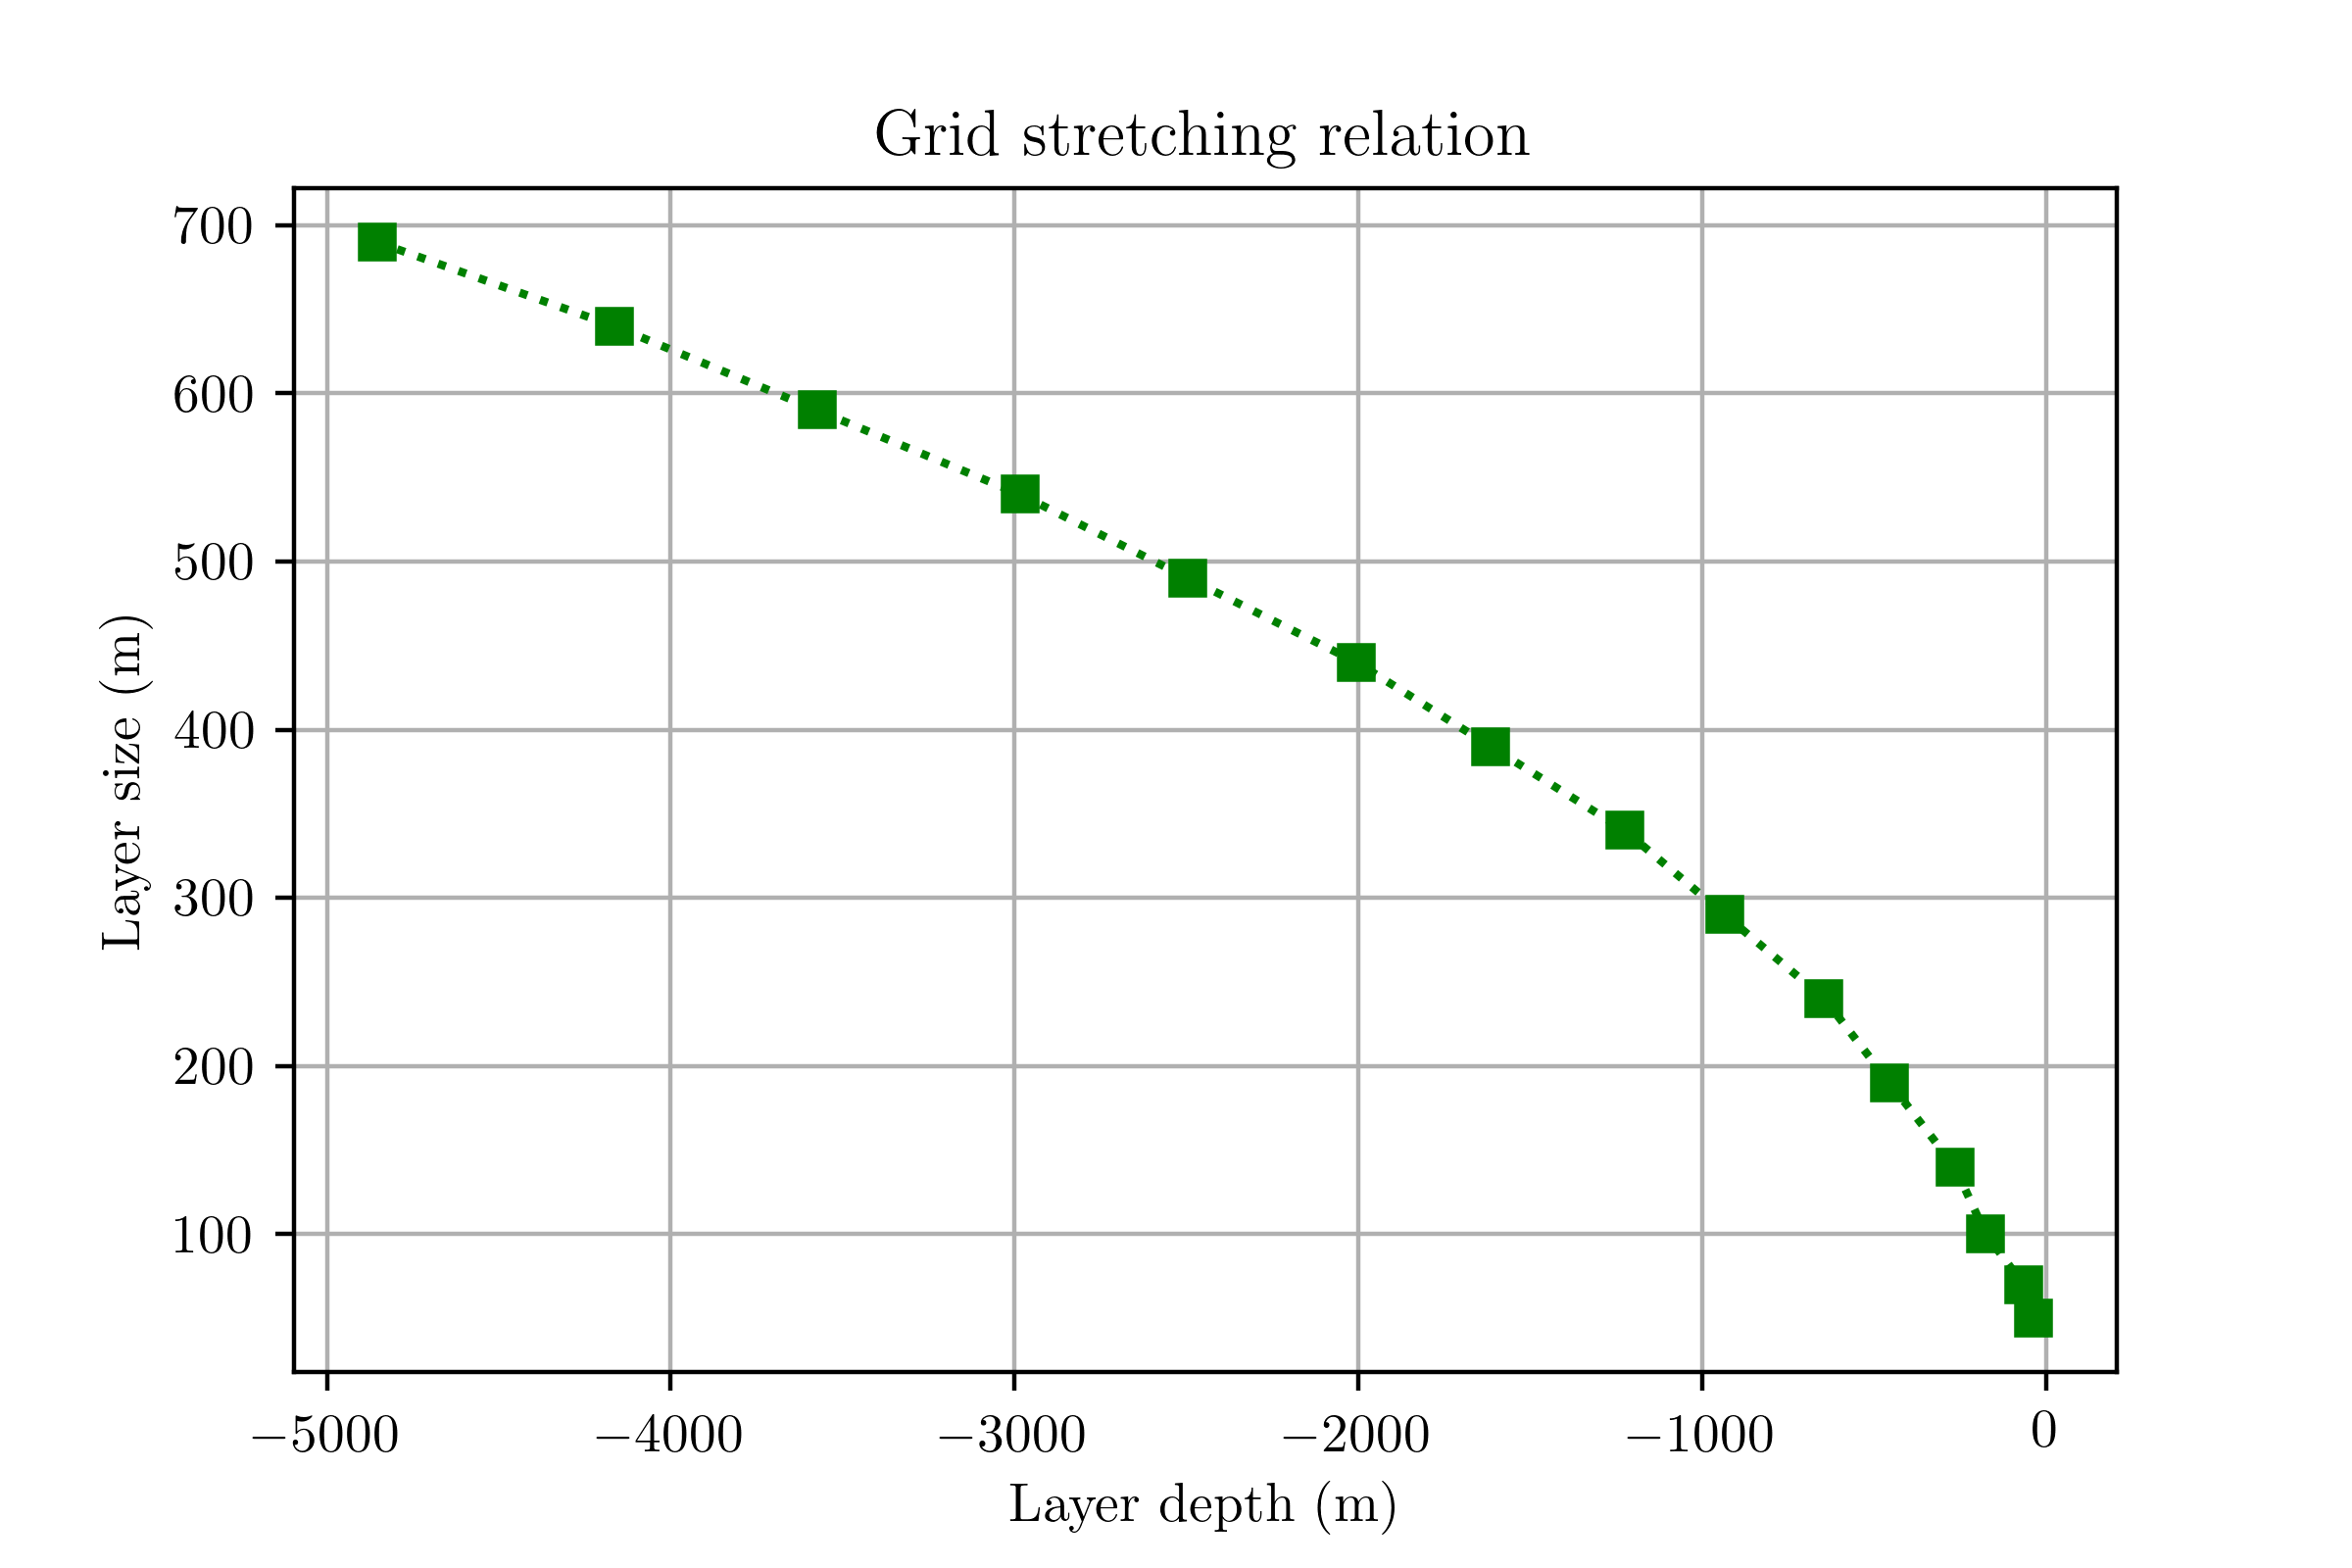
\includegraphics[width=\linewidth]{grid_stretching.png}
 	\caption{Figure of the grid stretching relation used.}
 	\label{fig:gridstrech}
 \end{figure}

\subsubsection{Surface Forcings}\label{sec:forcing_ideal}
The model used, uses restoring boundary conditions. Restoring the boundary at the surface of the oceanic basin to be a value based on a forcing field for Sea Surface Temperature (SST), Sea Surface Salinity (SSS), wind stresses ($\tau$) and heat flux.
Choosing the correct forcing for the ocean is very important. It is known that in general circulation models the MOC is highly sensitive to even small changes in surface forcings (\cite{Milliff1999May}). Attempts at making these forcings highly idealized have often been made in the past with varying rates of success(\cite{bryan1987parameter}; \cite{Mulder2017Jul}). We note the fact that using idealized forcings will probably induce the errors, especially in the shape of the thermohaline circulations. The use of idealized forcings is however justified here because we are only interested in large scale features of the AMOC and the wind-driven circulations.

Several methods are explored when it comes to creating these idealized forcings. In the \cite{Mulder2017Jul} paper an analytic forcing profile was used for wind stress, SST, and SSS (\cref{fig:idealized_forc}). Veros is however a seasonally forced model. Using these simplified forcings would thus fail to capture seasonal changes especially in the SST. There have been studies suggesting that these seasonal forcings can have large effects on the strength of the meridional overturning circulation (\cite{schmittner2001seasonally}). Here we propose to take the SSS and SST profiles as zonal means of realistic forcings. We use $1^{\circ} \times 1^{\circ}$ forcings from the ECMWF public dataset a basis (\cite{ECMWFForc}). While the zonal wind stress is set to the simple profile proposed by \cite{bryan1987parameter}. The choice of this analytic profile was made over a zonally averaged forcing mirrored along the equator ($\mu(\tau_x)$). These were both tested on the present-day configuration to see which of these forcings most accurately captures the present-day MOC. After some initial tests, we found that $\mu(\tau_x)$ is very weak in the sub polar regions and subsequently fails to force the North Atlantic Deep Water formations (NADW).
\end{multicols}
%example full width overturning

\begin{figure}[H]
\begin{subfigure}{.5\textwidth}
	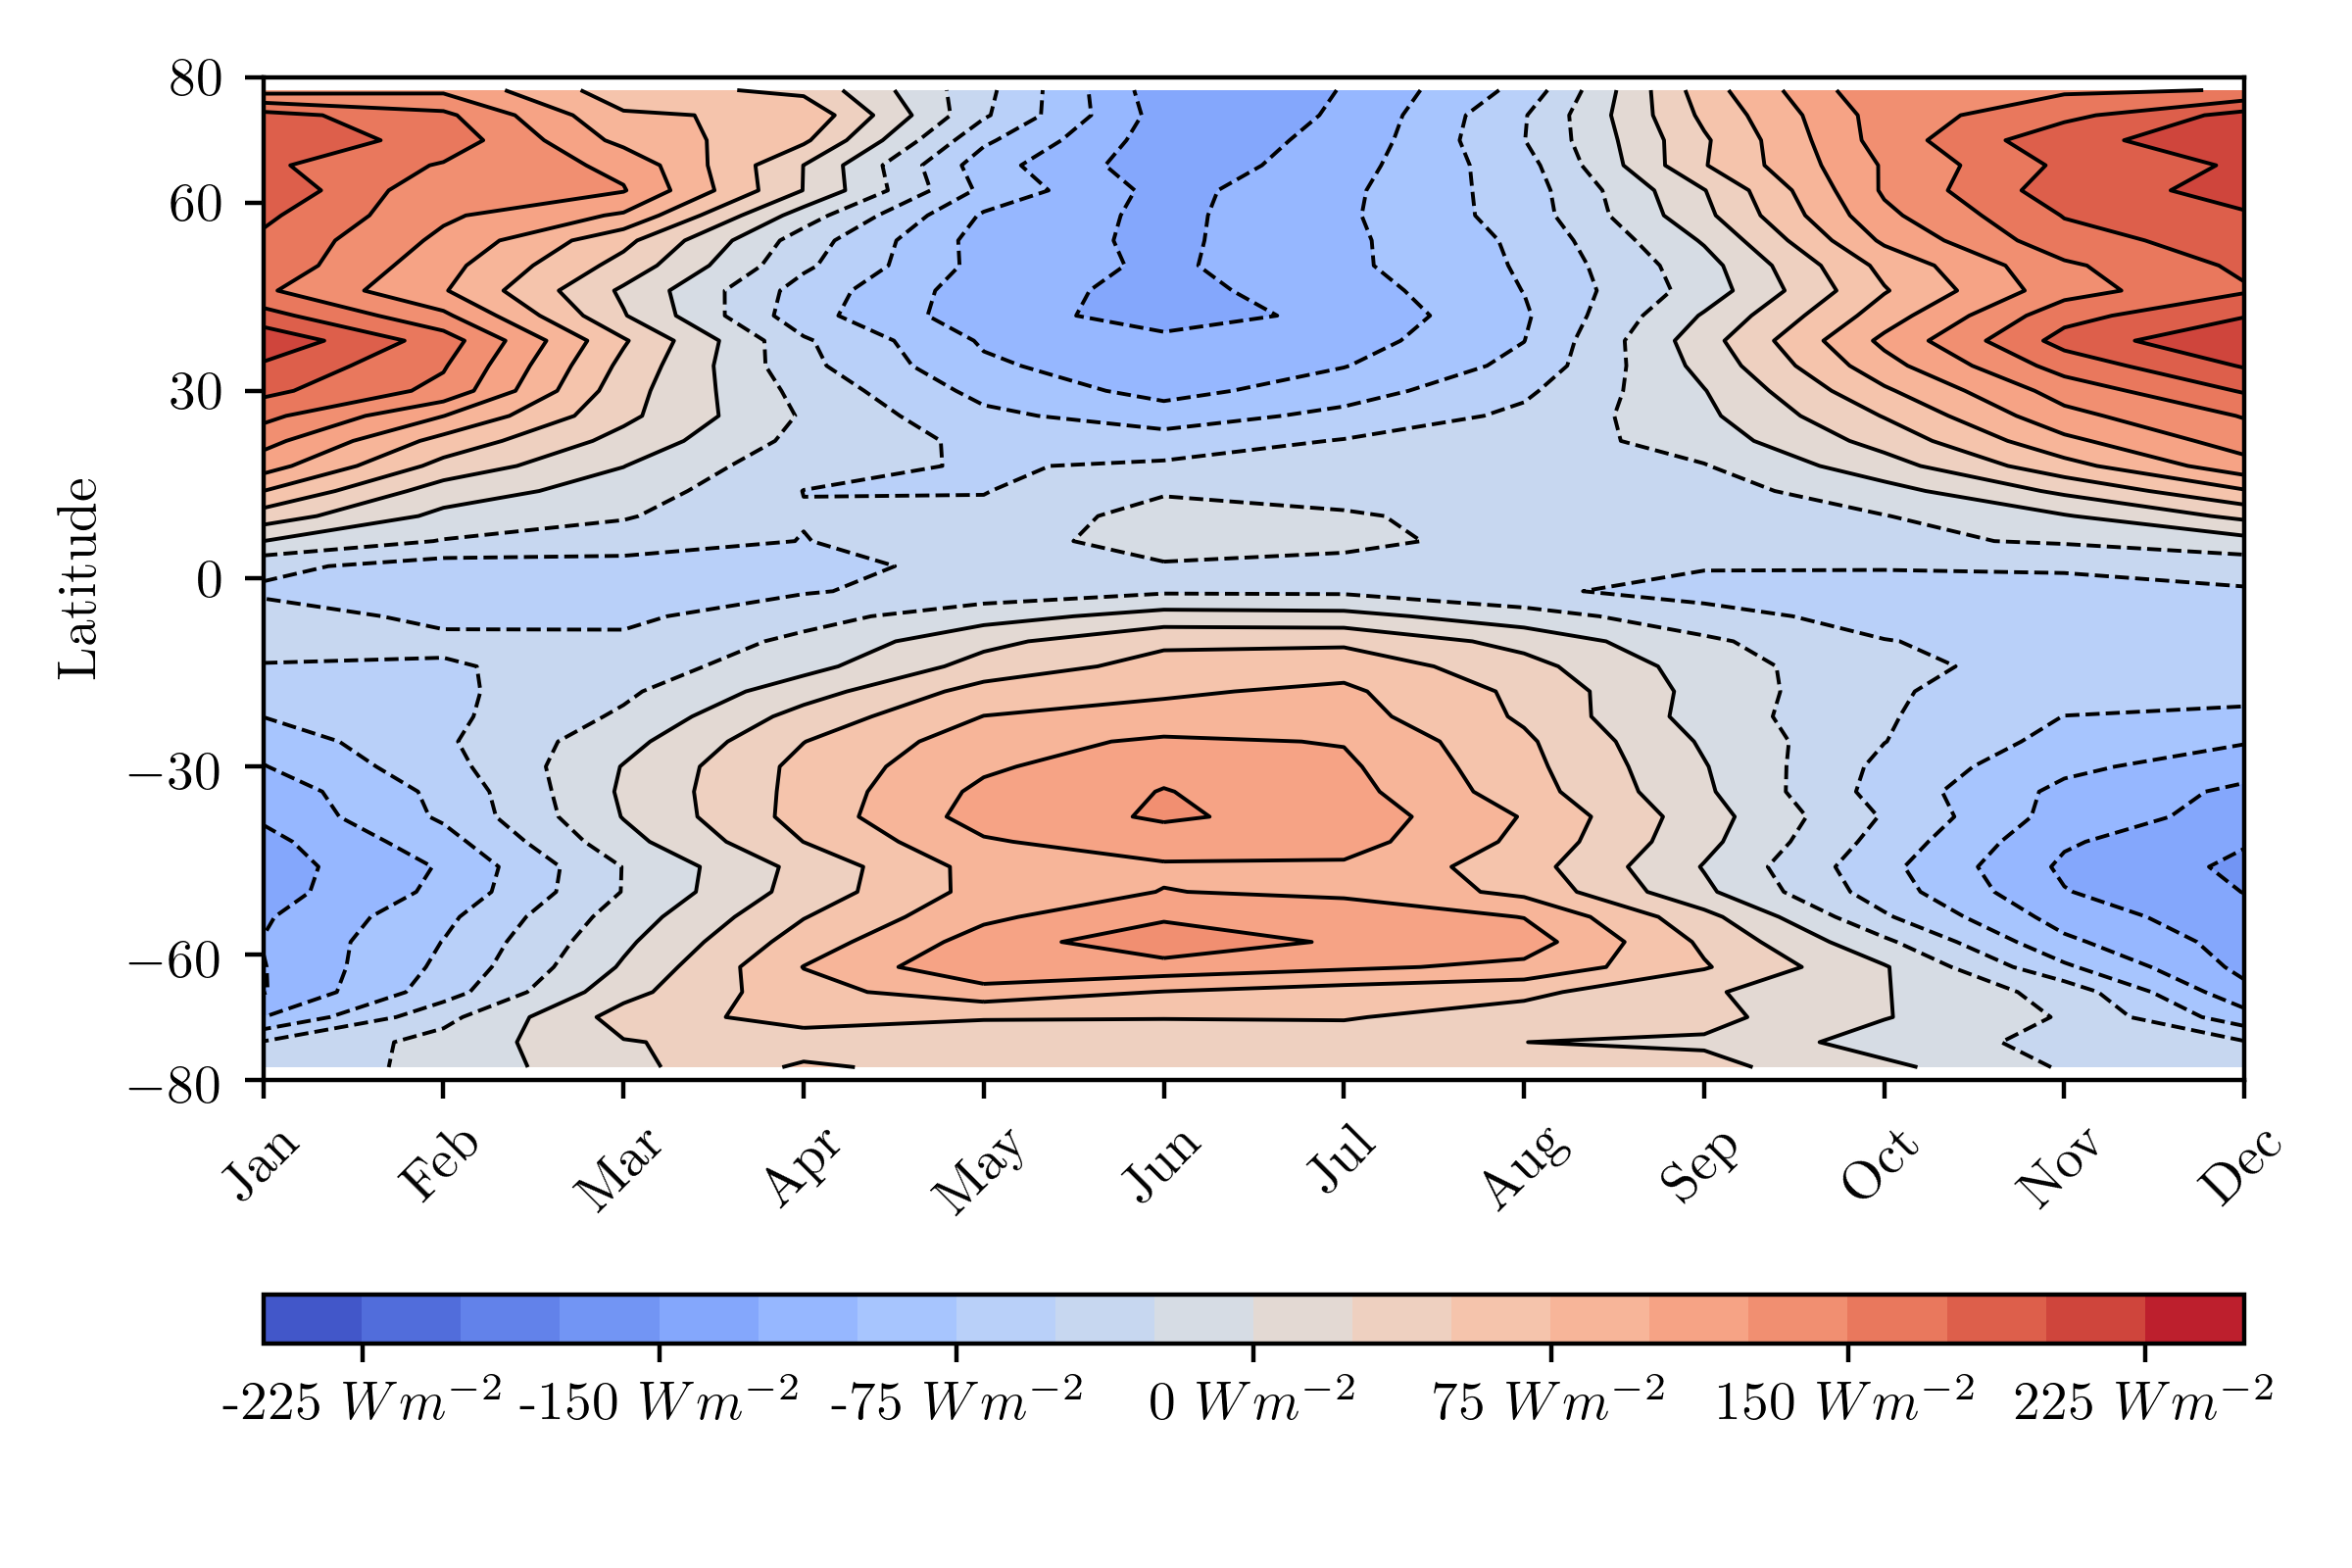
\includegraphics[width=\linewidth]{q_net_profile.png}
	\caption{Net Heat flux}
	\label{fig:qnet}
\end{subfigure}
\begin{subfigure}{.5\textwidth}
	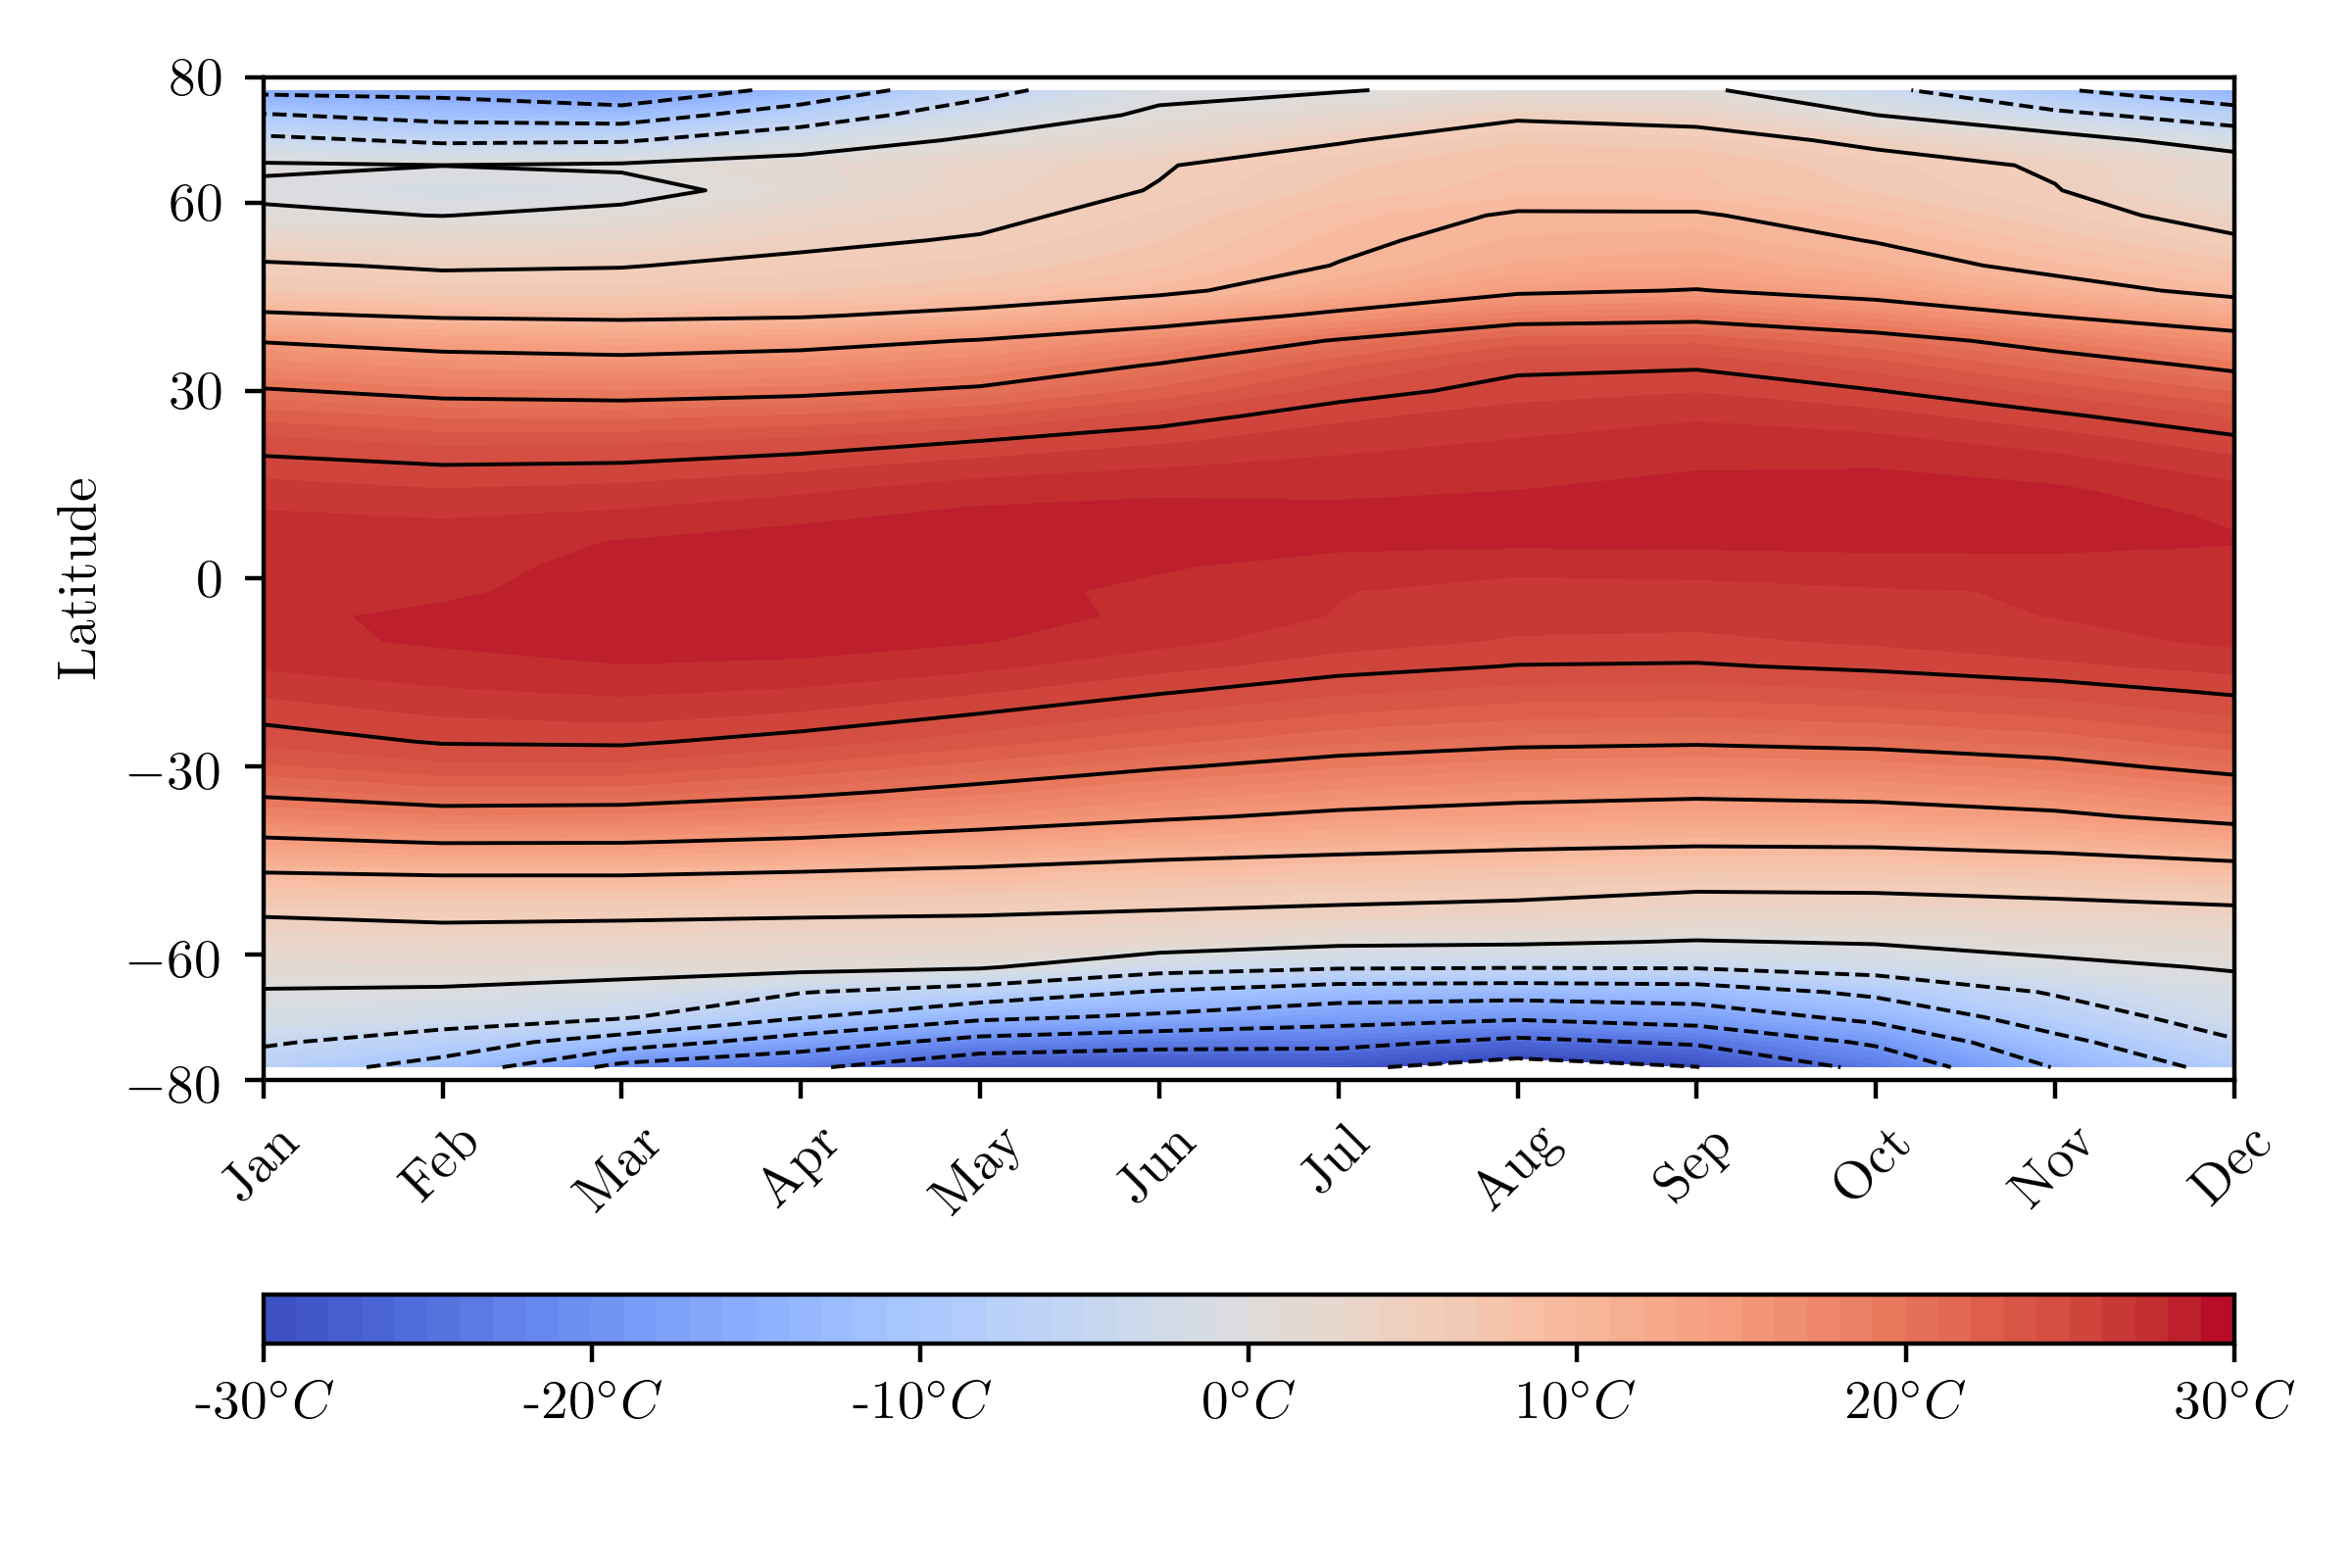
\includegraphics[width=\linewidth]{sst_profile.png}
	\caption{SST profile}
	\label{fig:sst_profile}
\end{subfigure}
\begin{subfigure}{.5\textwidth}
	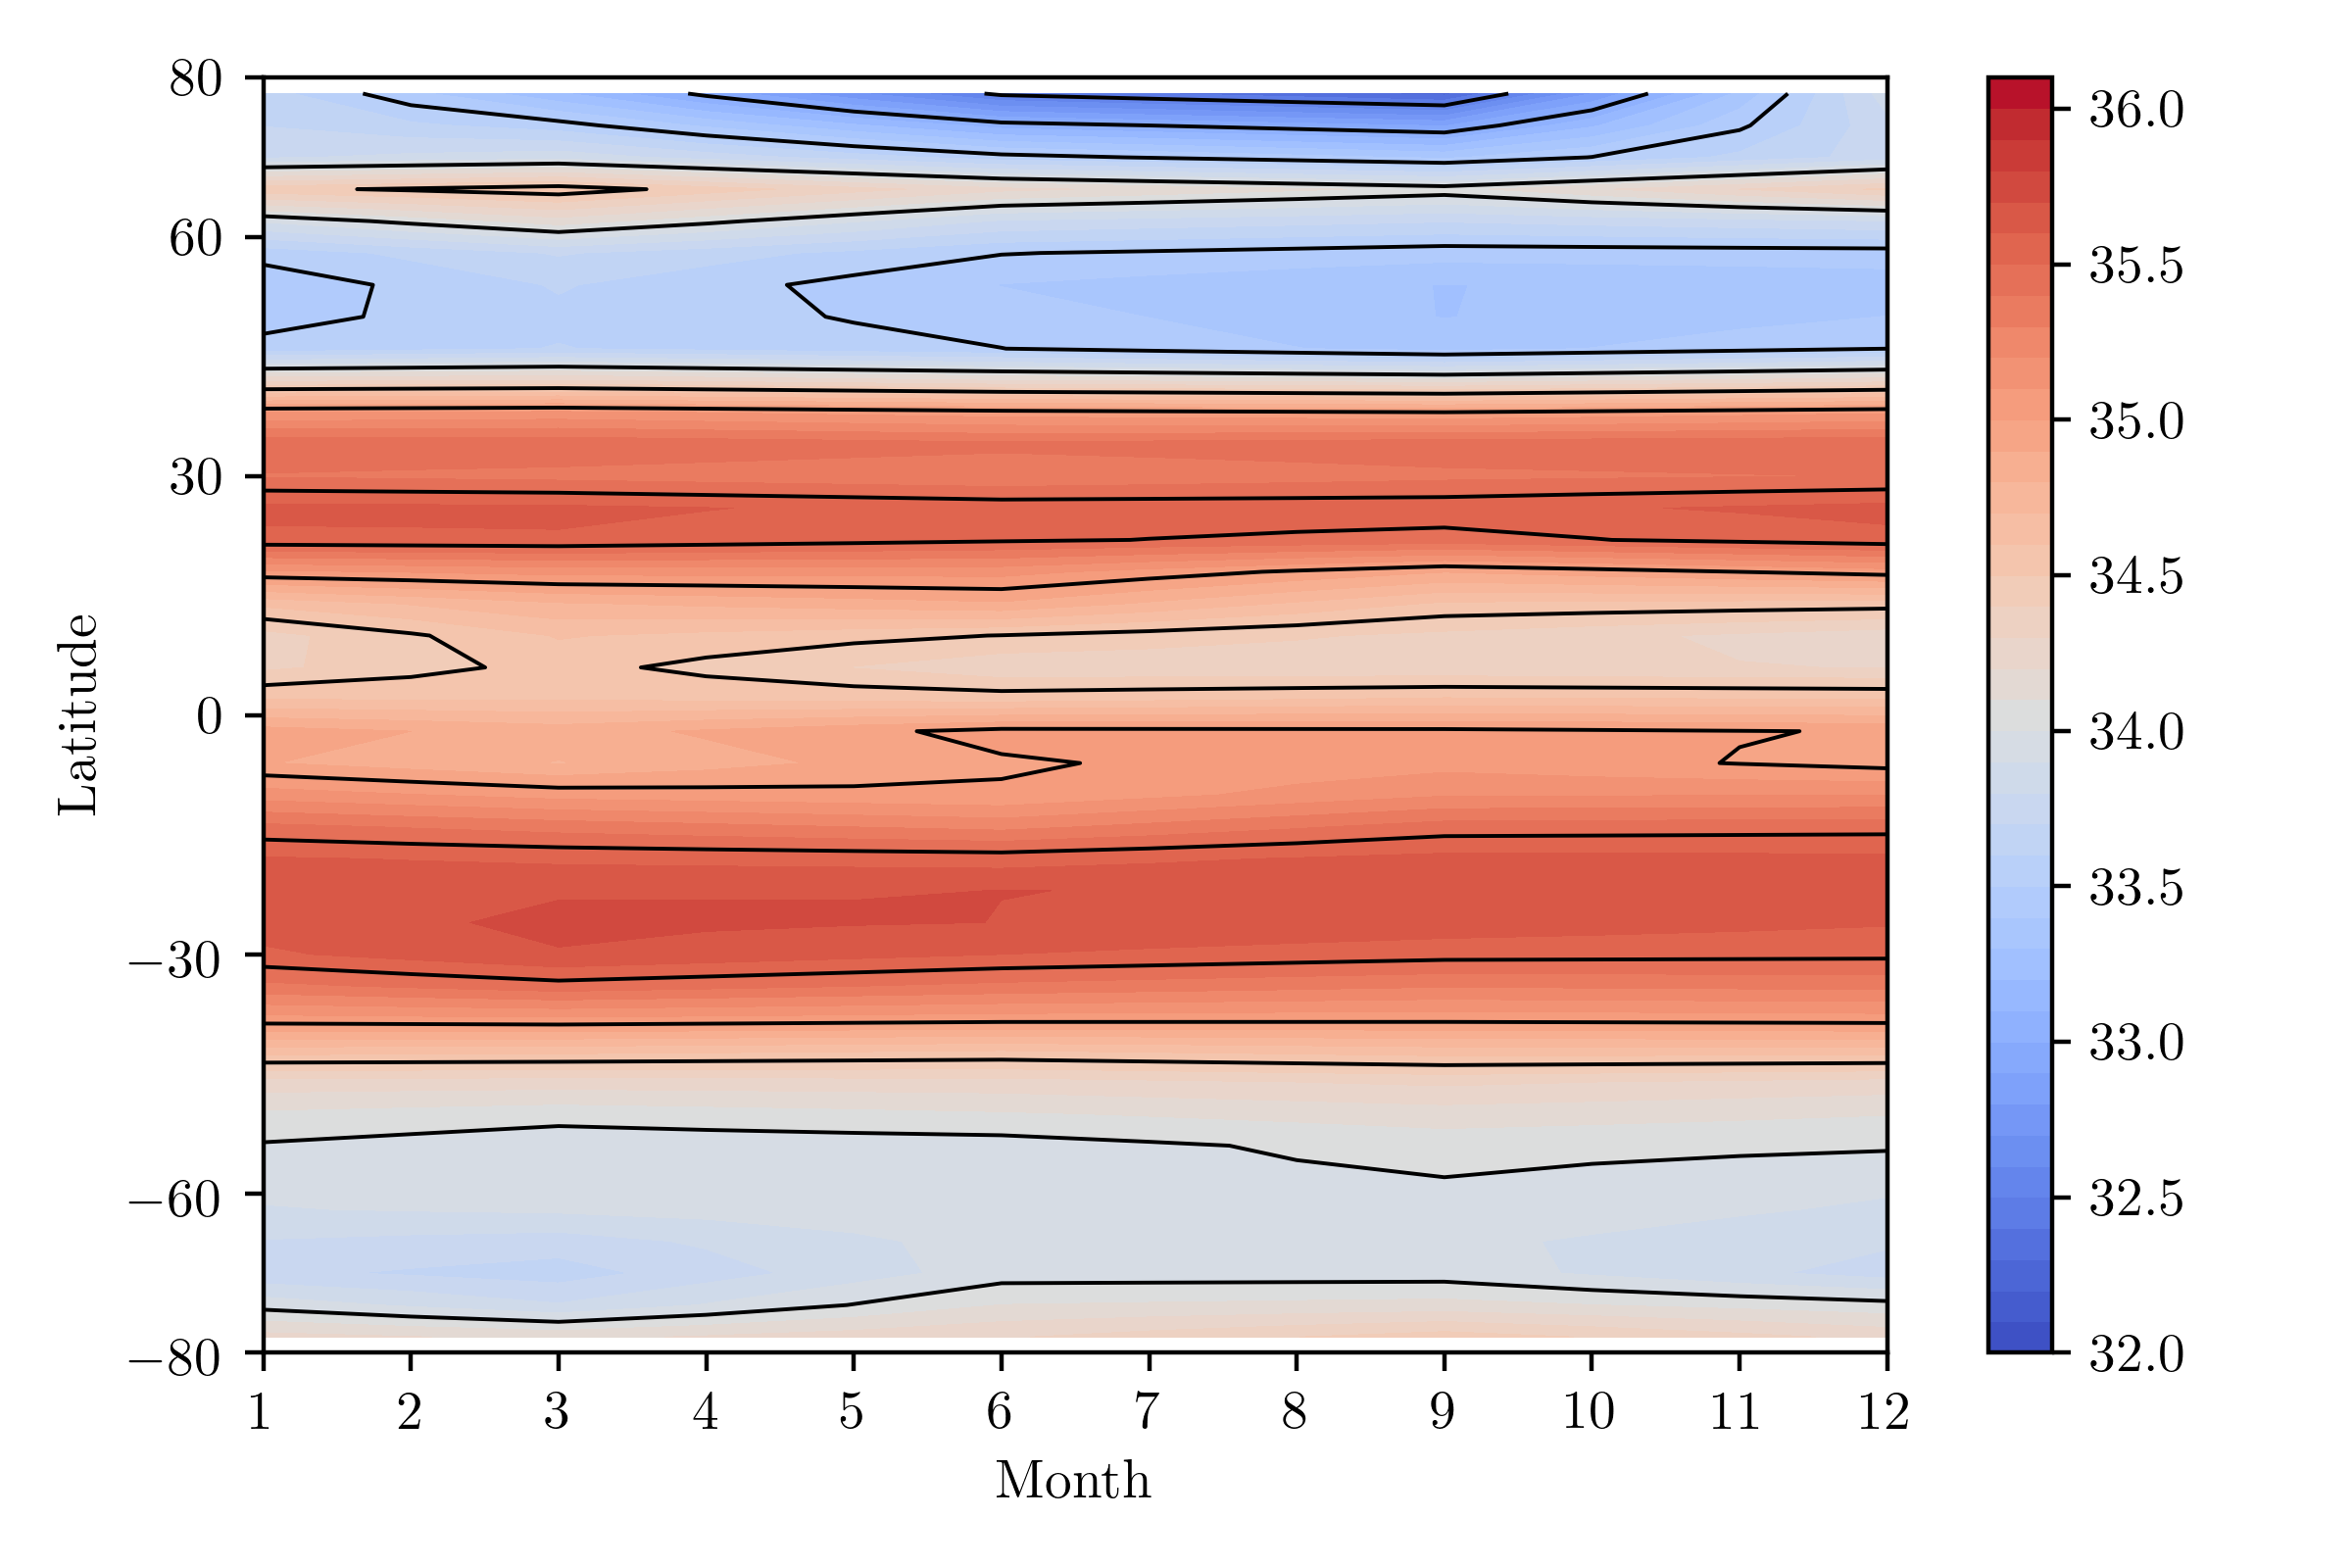
\includegraphics[width=\linewidth]{sss_profile.png}
	\caption{SSS profile}
	\label{fig:sss_profile}
\end{subfigure}
\begin{subfigure}{.5\textwidth}
	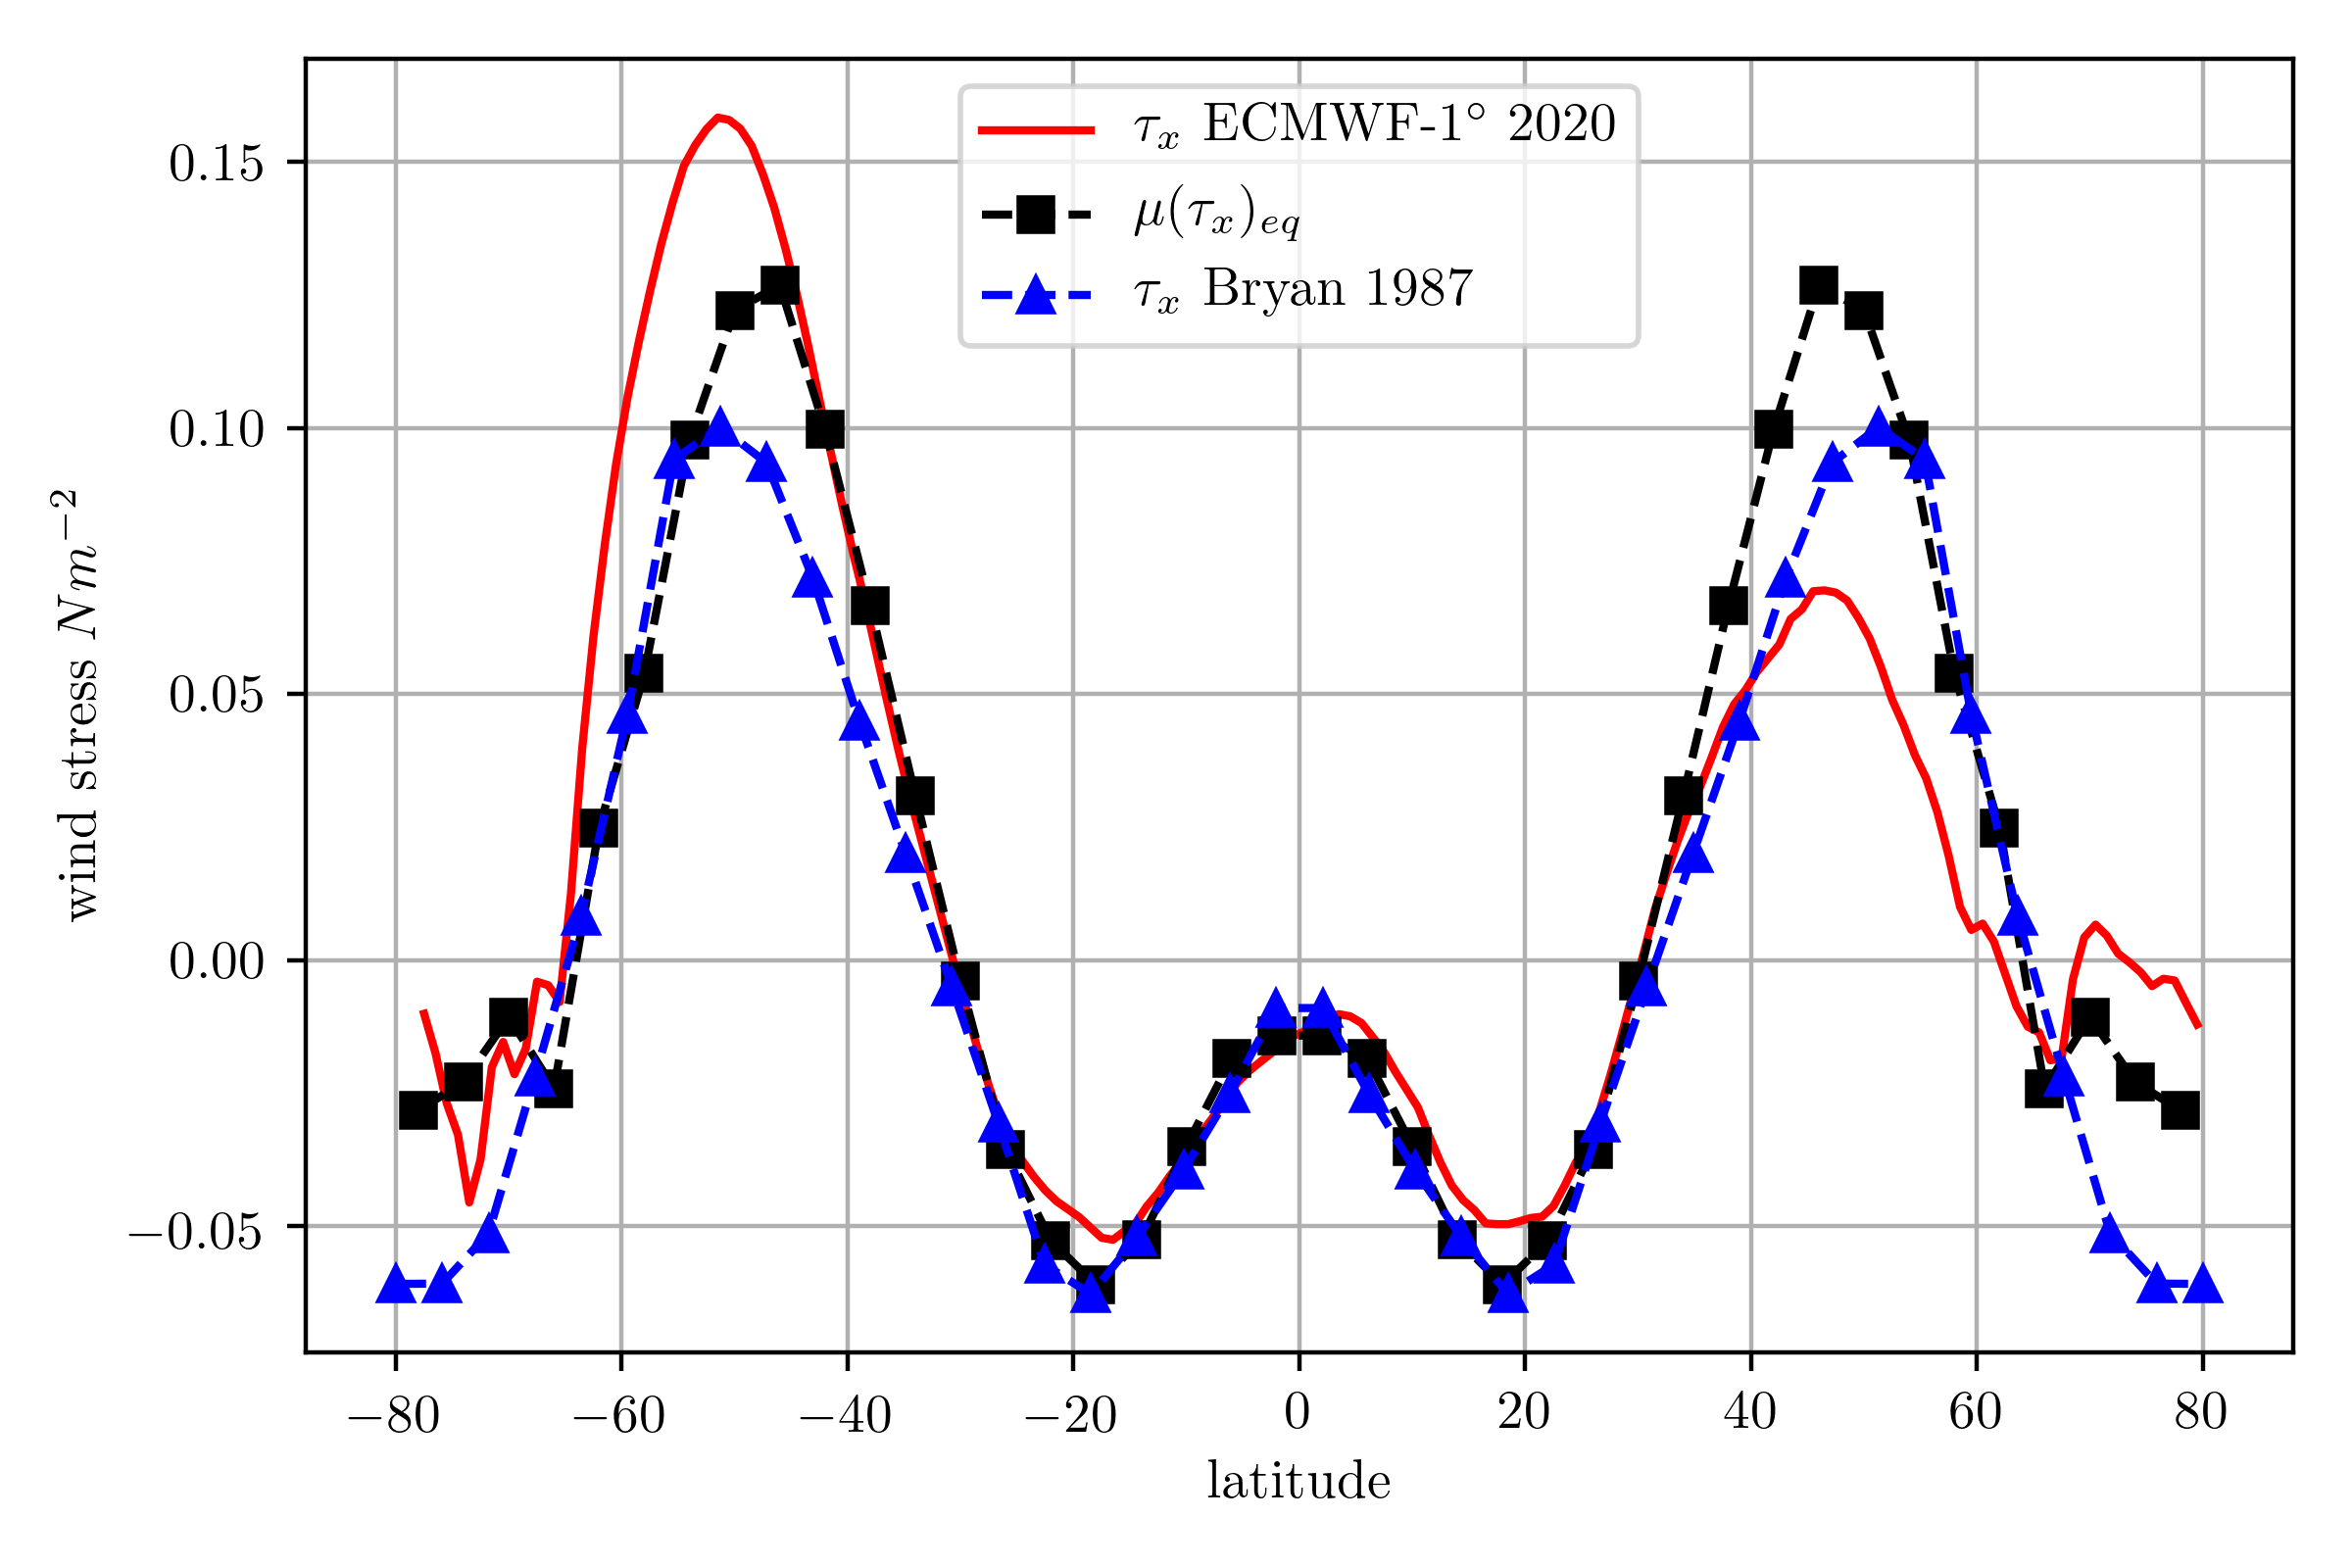
\includegraphics[width=\linewidth]{windstress_models.png}
	\caption{$\tau_x$ profile}
	\label{fig:tau_profile}
\end{subfigure}
%\begin{subfigure}{.5\textwidth}
%	\centering
%	% include first image
%	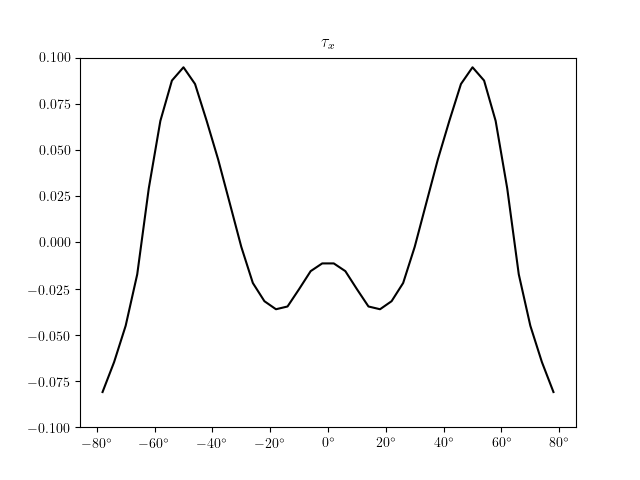
\includegraphics[width=0.9\linewidth]{tau_x_profile.png}
%	\caption{Zonal wind stress ($\tau_x$) profile}
%	\label{fig:tau_X}
%\end{subfigure}

\caption{Idealized forcing profiles for \textbf{a)} The net heat flux, \textbf{b)} The Sea surface Temperature }
\label{fig:idealized_forc}
\end{figure}

\begin{multicols}{2}
 \subsubsection{Forcing bias} \label{sec:forc_err}
The forcings we use here have large errors compared to reality. This can be seen if we compare the original realistic forcings to the zonal mean of these forcings. In \cref{fig:sss_sst_errors} the errors compared to present-day forcings are shown. there is a particularly large discrepancy in the Atlantic, which has a much higher salinity in reality than in our forcing. This may have implications on the thermohaline circulation we will observe in our model. It is furthermore noted that the northern Atlantic ocean is much warmer in reality than in our model, which again possibly can affect the thermohaline circulation.
We also note that the temperature on earth was also much higher in the early part of the 65Ma period (\cite{Hansen2013Oct}). We neglect this effect because we use the same forcing for each time step. Therefore, it is not possible to compare our results directly with existing proxies. However, studying the effect of geography changes specifically is much clearer using this method.

\end{multicols}
\begin{figure}[H]
	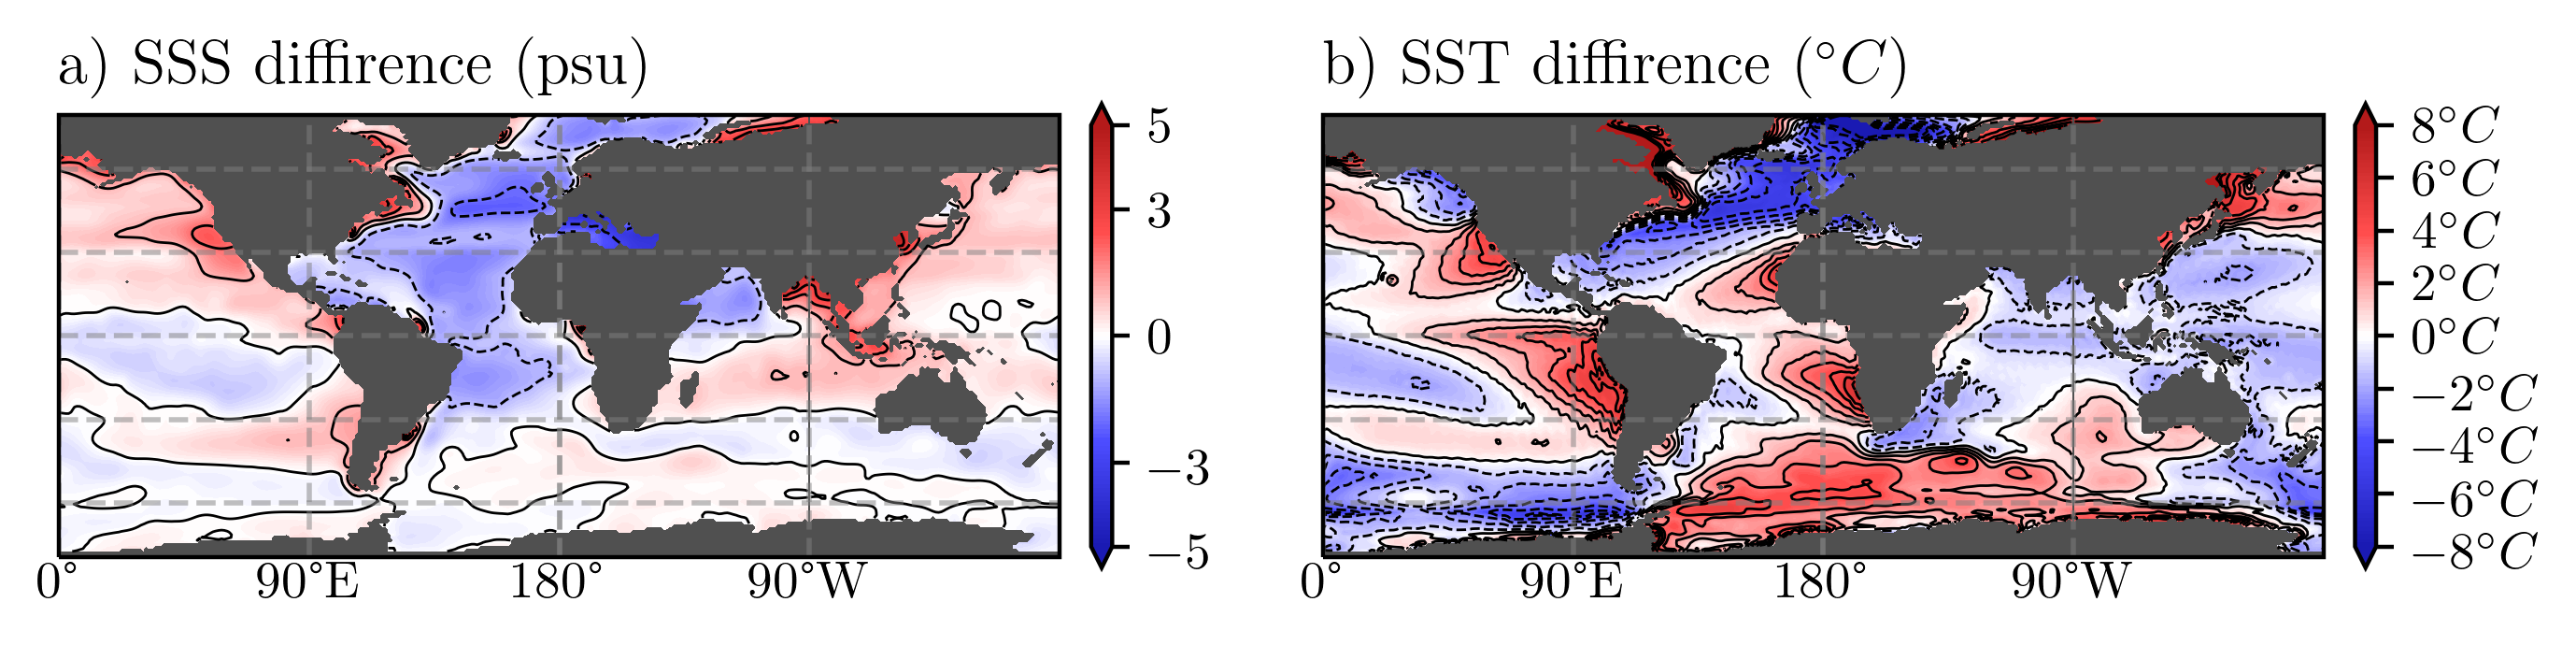
\includegraphics[width=\linewidth]{SST_SSS_errors.png}
	\caption{Figure showing errors in surface forcing. As a diffirence between ECMWF forcings and zonal mean forcings. As a monthly average. Here positive values are over estimations of realistic forcings. Errors for: \textbf{a)} the SSS difference with contours every 1 psu and \textbf{b)} the SST difference with contours every 1 $^{\circ}C$}
	\label{fig:sss_sst_errors}
\end{figure}
\begin{multicols}{2}
 \subsubsection{Initial conditions}
The model is started with an initial temperature and salinity profile that is, like the forcings taken from observational data (\cite{ECMWFForc}). The temperature profiles again use zonal means. This results in the profile seen for the situation around the equator in \cref{fig:salt_temp_prf}.

\begin{figure}[H]
	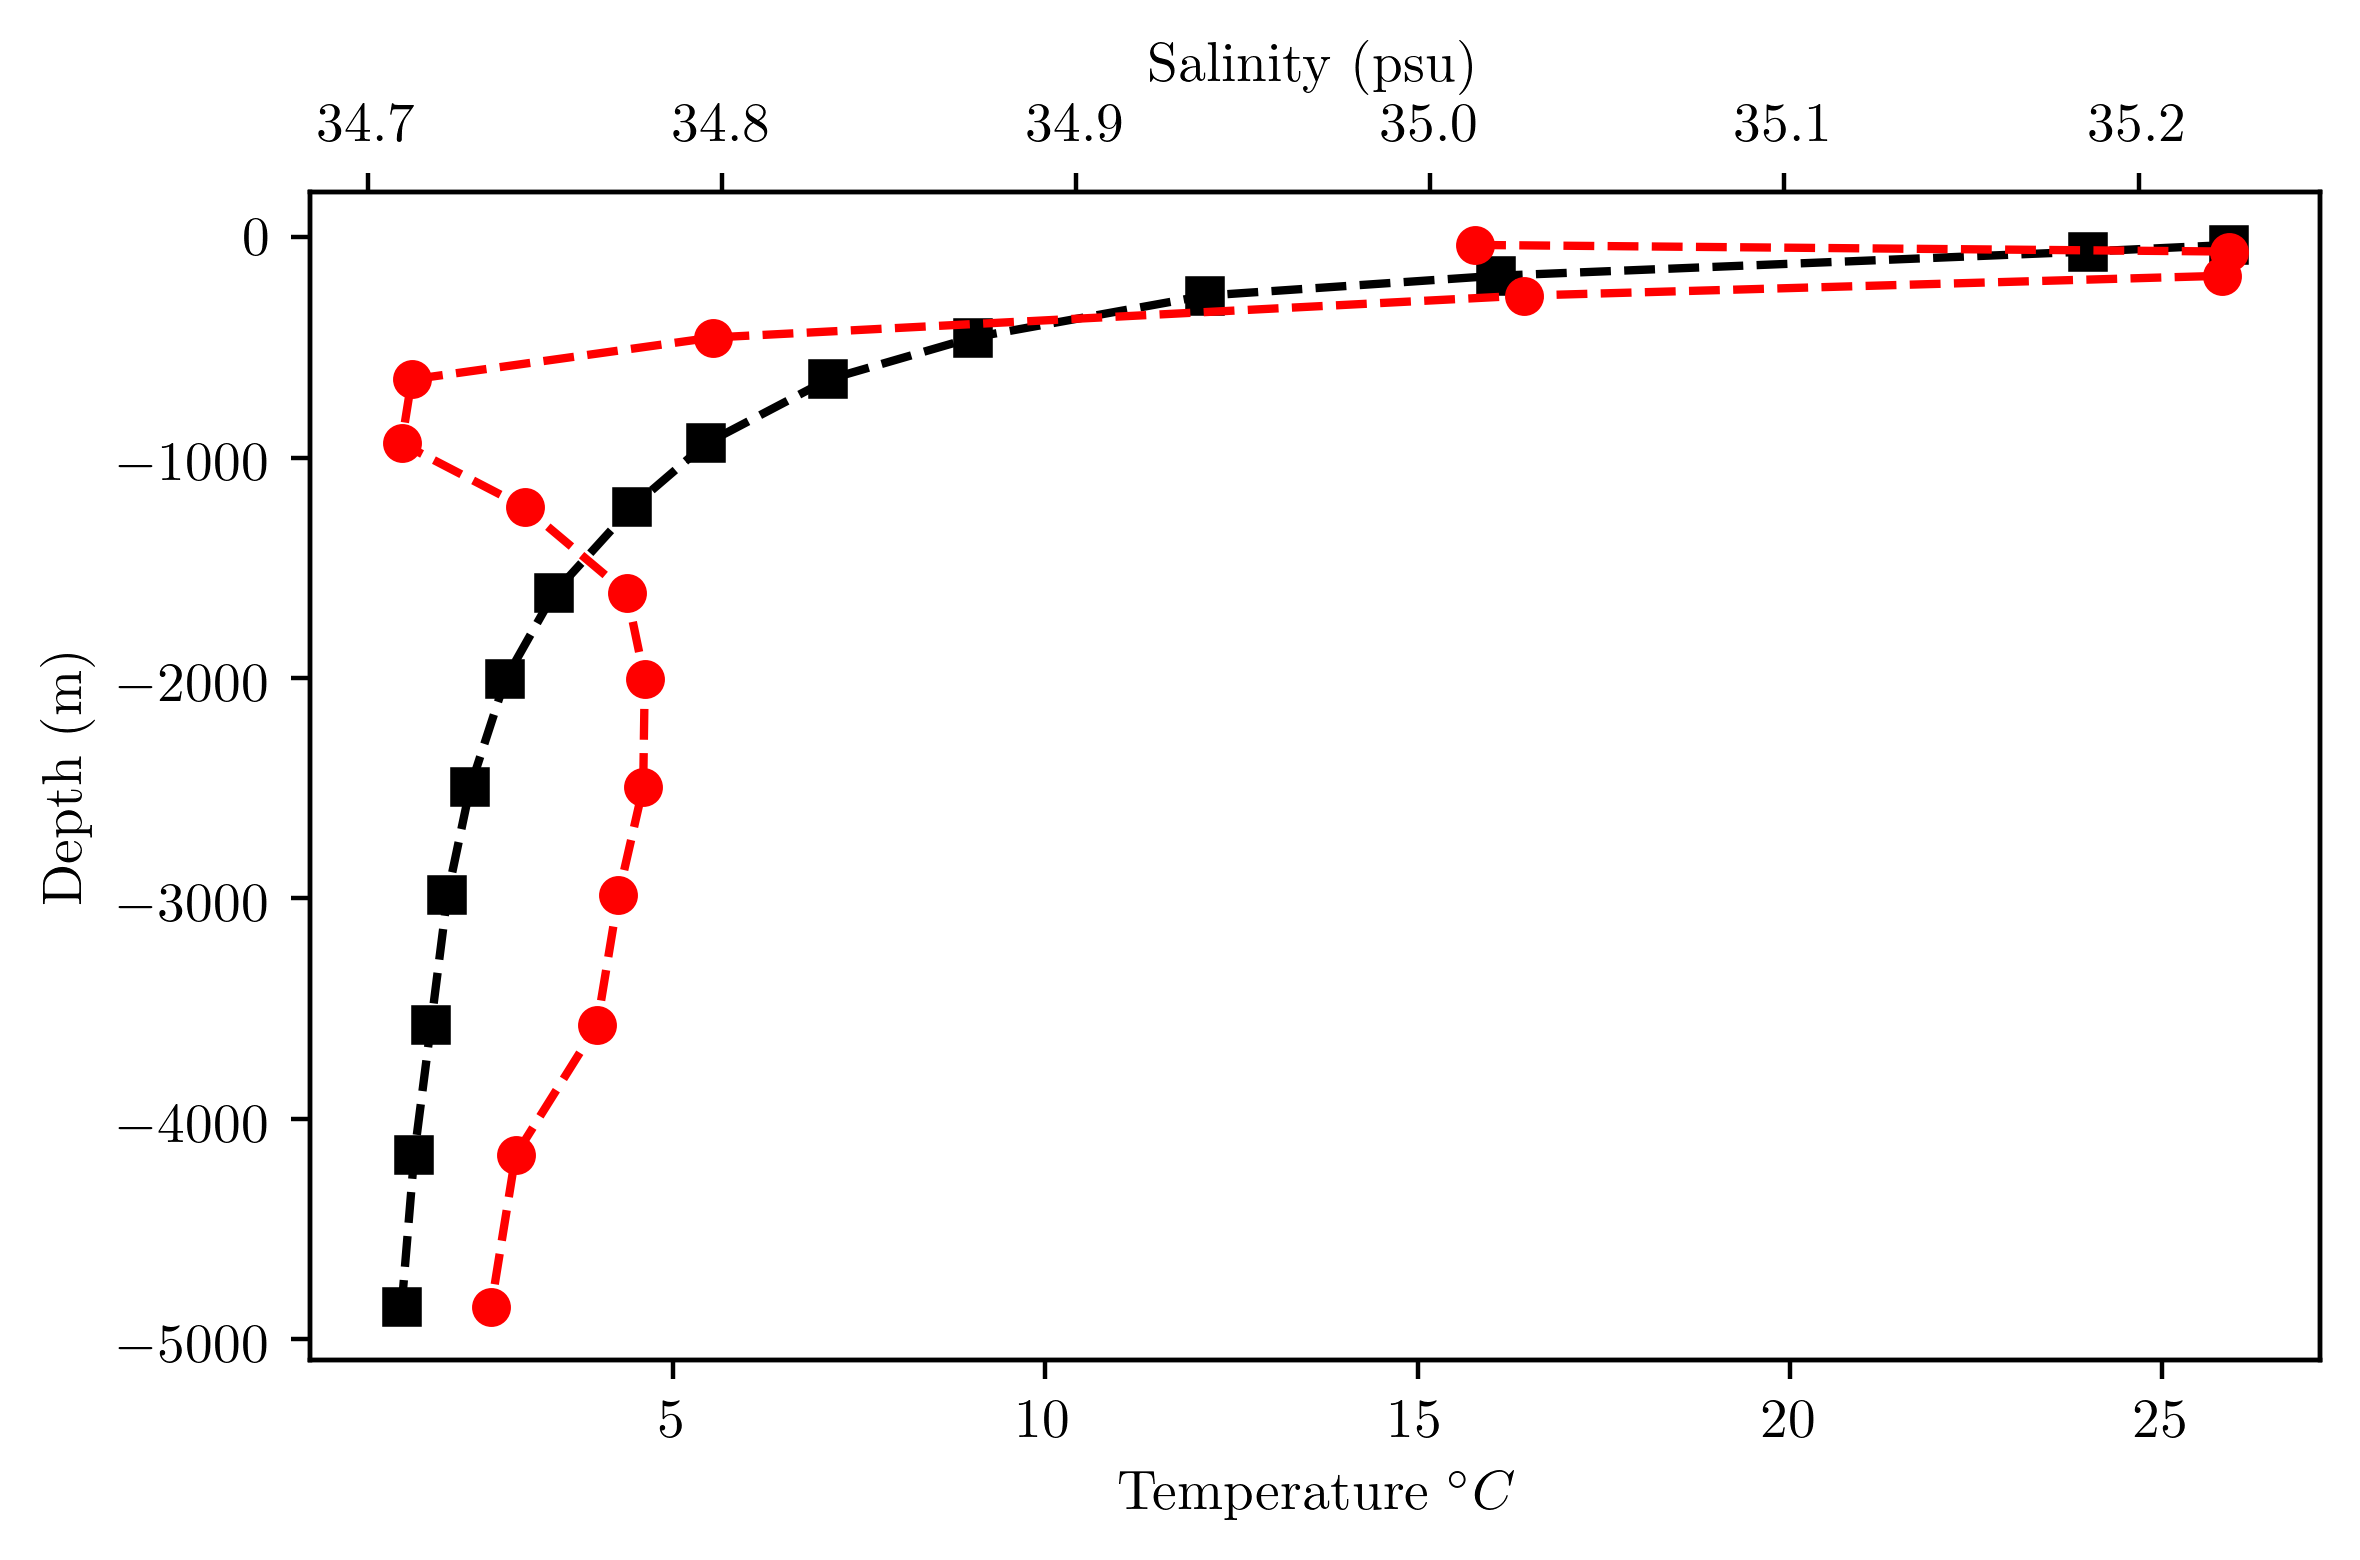
\includegraphics[width=\linewidth]{salt_temp_prof.png}
	\caption{Figure showing the temperature and salinity profiles at $2^{\circ} N$. Black squares indicate the Temperature profile and red circles indicate the salinity profile.}
	\label{fig:salt_temp_prf}
\end{figure}
 
 \subsubsection{MOC stream function} \label{sec:MOCSTREAM}
 

The global Meridional Overturning Circulation $\Psi_{MOC}$ is defined as the zonally integrated meridional volume transport of water in the worlds oceans. It can be written down as:

$$
\Psi_{MOC}(y,z) = \int_{z}^{0} \int_{-180^{\circ}}^{180^{\circ}} v(x,y,z') dx dz'.
$$
Here $v$ is the meridional component of the velocity.
$ \Psi_{MOC}$ is thus a stream function of the zonally integrated volume transport in the Earth's ocean basins. Plotting this stream function can give a lot of insight into the deep water transport associated with the thermohaline circulation. In this paper, we hope to capture these deepwater transport formations. In particular, we are looking for the shape of the North Atlantic deep water (NADW) and the Antarctic Bottom Water (AABW) formations.

 \begin{figure}[H]
	\includegraphics[width=\linewidth]{moc_example.png}
	\caption{Meridional overturning circulation with schematic arrows indicating flow direction. Also including general areas of flow. AABW: Antarctic Bottom Water, NADW: North Atlantic Deep Water, NPIW: North Pacific Intermediate Water,  PWD: Pacific Deep Water, IDW: Indian Deep Water, SAMW: Subantarctic Mode Water, AAIW: Antarctic intermediate Water, ACC Antarctic Cicumpolar Current. MOC taken from \cite{Forget2015Oct}.}
	\label{fig:moc_ex}
\end{figure}

\subsubsection{Barotropic Stream Function} \label{sec:BSF_theory}
It is furthermore interesting to look at an expression for the transport of ocean gyres. We know that the depth-integrated flow must be horizontally non-divergent. Thus a stream function $\Psi_{b}$ can be introduced. Where $v(x,y,z)$ is the meridional velocity:
\begin{align}
U = -\frac{\partial \Psi_{b}}{\partial y}; V=\frac{\partial \Psi_{b}}{\partial x} \\
\Psi_{b}(x, y) = \int_{eastern bdy}^{x} \int_{-D}^{0} v(x',y,z) dz dx'
\end{align}

This so-called barotropic stream function $\Psi_{b}$ is defined by integrating the meridional transport westward from the eastern boundary of the domain. It is a useful tool to look at the shape and gyres associated with the major ocean current systems. By using the Sverdrup relation
$$
\int_{-D}^{0}v(x,y,z) dz = \frac{1}{\beta \rho_{ref}}\vec{\hat{z}}\cdot \nabla \times \tau
$$

first proposed by \cite{sverdrup1947wind} we can look at a schematic diagram of the barotropic stream function based on the prevailing zonal winds. \cref{fig:schem_currents} shows a schematic of this relation. It is easily visible how the prevailing zonal winds relate to the wind stress forcing seen in \cref{fig:idealized_forc}. The calculation of the barotropic stream function without easily defined boundaries is quite a bit more cumbersome than a simple integration from the eastern boundary. Veros uses a process in which special treatment is given to boundaries using something called island integrals. This is why the barotropic stream function has values below the land mask in Veros. 
 
  \begin{figure}[H]
 	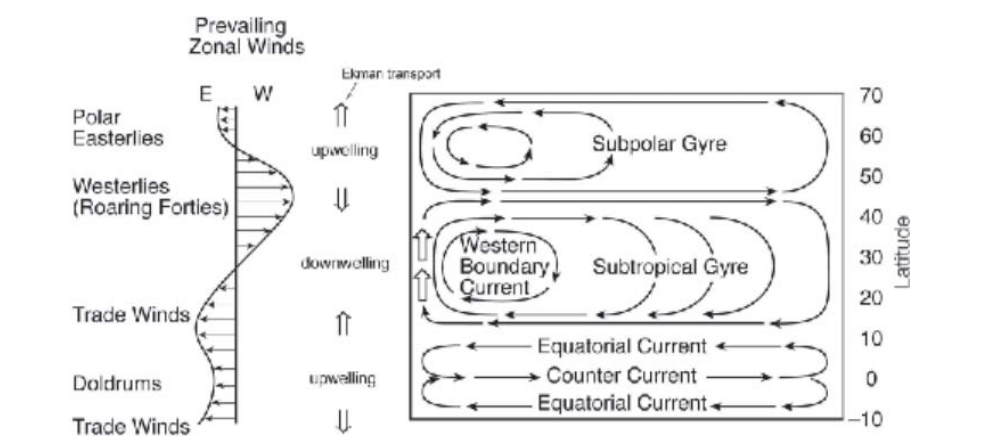
\includegraphics[width=\linewidth]{schematic_marshall_plumb.png}
 	\caption{Schematic of the barotropic stream function based on the Sverdrup relation. Showing the subpolar and subtropical Gyres and equatorial currents. Figure taken from \cite{MarschallPlumb}}
 	\label{fig:schem_currents}
 \end{figure}
\subsubsection{Passage throughflow}\label{sec:throughflowp}
For each of the passages mentioned in \cref{sec:bathys} it is interesting to talk about the total volume transport through each of the passages discussed. The volume transport in the zonal direction through an area $A$ is defined as 
\begin{align}
Q = \iint_A v(x,y,z) dA.
\end{align}	
Here we integrate the zonal velocity over an area $A$ in the latitude-vertical direction that is normal to this velocity. We can thus use the output of the BSF $\Psi_b$ to find the zonal volumetric flux through each grid cell in our model.

For each passage a suitable location is chosen such that there are no boundaries next to the passageways, this is done for each time step. This method is the same for each of the passages and thus we can study the effect of changes in bathymetry to on the relative strength of the flow. However, it should be noted that these values may not represent real physical values. As the passages in a $4^{\circ}$ model are often only a few grid cells wide. Resulting in discrepancies in the calculation of the throughflow due to boundary conditions. We do however expect mass to be conserved and thus that the throughflow in each ocean adds up to 0. In \cref{fig:passages_ocean} An overview is shown of all the passages discussed in this paper. 


\end{multicols}
 \begin{figure}[H]
	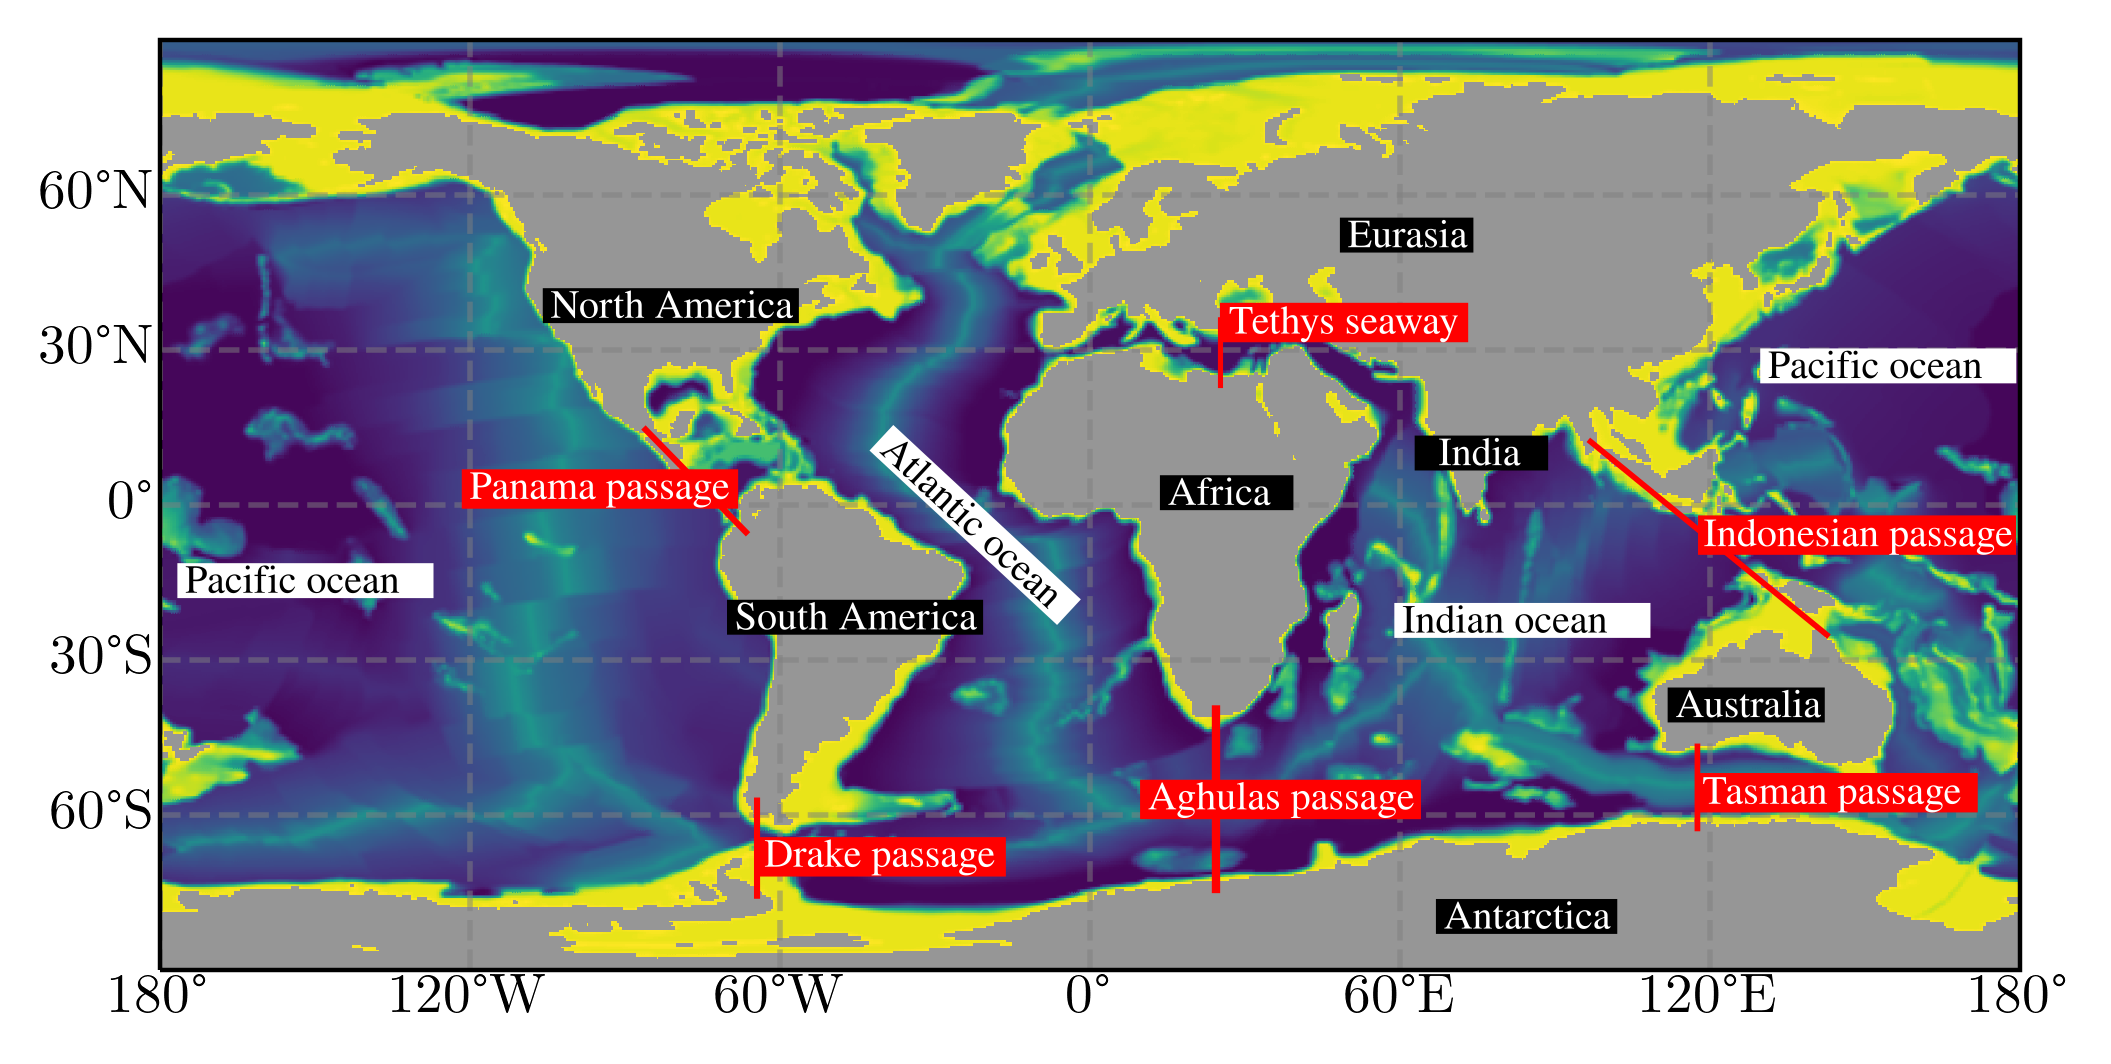
\includegraphics[width=\linewidth]{passages_oceans.png}
	\caption{Schematic image showing the 30 Ma bathymetry in $0.5^{\circ} \times 0.5^{\circ} $. Overlayed in red are the passages we study. In black the continents and in white the oceanic basins.}
	\label{fig:passages_ocean}
\end{figure}
\begin{multicols}{2}